\appendix
\section{SM}


\subsection{Derivatives of the Partition Function}\label{Z-to-macros}

\subsection{MFT Expansion about the critical temperature}\label{sec:mft-expansion}
To show this, let us approximate a solution in the
vicinity of the critical point. We will Taylor-expand the $\tanh$ in
the vicinity of the critical point ($\b J n = 1; \bar{s}=0$) using
$\tanh(x)= x- x^3/3+\mc{O}(x^5)$:%
\begin{align}%
  \bar{s}&\approx \b J n \bar{s}- \frac{1}{3}{(\b J n \bar{s})}^3\\
  \implies \bar{s}&\approx \root{2}{\frac{3(1-\b J n)}{(\b J n)^3}}.
\end{align}.%

\subsection{Exact Solution of 1D Ising Model: The Transfer Matrix
  Method}\label{sec:ising-1d-exact}

Restricting to the 1-D case, we can simplify matters by taking the
boundary conditions of our lattice to be periodic
($s_{N+1}=s_{1}$)\footnote{This is perfectly acceptable in the limit
  $N\rightarrow 0$}. Note that we can rewrite the 1D Ising energy
function~(\ref{}) as follows:
\begin{equation}%
  E(\bs)=-\sum_i^N \left(J s_i s_{i+1} + \frac{B}{2}(s_i + s_{i+1})\right)
\end{equation}%
We manipulate the partition functions:
\begin{align}%
  Z&=\sum_{\bs\in\mc{S}}e^{-E(\bs)}\\
   &=\sum_{s_1\in\{-1,1\}}\dots \sum_{s_N\in\{-1,1\}}e^{\sum_i^N \left(J s_i s_{i+1} + \frac{B}{2}(s_i + s_{i+1})\right)}\\
   &=\sum_{s_1\in\{-1,1\}}\dots \sum_{s_N\in\{-1,1\}}\prod_i^N e^{\left(J s_i s_{i+1} + \frac{B}{2}(s_i + s_{i+1})\right)}\\
   &=\sum_{s_1\in\{-1,1\}}\dots \sum_{s_N\in\{-1,1\}}\prod_i^N p_{s_i,s_{i+1}}\\,
  \label{eq:partition-decomposition-1d}
\end{align}%
where
$p_{s_i,s_{i+1}}\equiv e^{\left(J s_i s_{i+1} + \frac{B}{2}(s_i +
    s_{i+1})\right)}$. These $p_{m,n}$ are such that:%
\begin{equation}%
  p_{1,1}=e^{J+B};\tab p_{1,-1}=p_{-1,1}=e^{-J};\tab p_{-1,-1}=e^{J-B}.
\end{equation}%
We use these to define the transfer matrix $\bT$:
\begin{equation}%
  \bT=
  \left[
    \begin{matrix}
      p_{1,1} & p_{1,-1} \\
      p_{-1,1} & p_{-1,-1}
    \end{matrix}
  \right]
\end{equation}%
We know from linear algebra that%
\begin{equation}%
  (bolds{T}^2)_{ij}=\sum_k \bT_{ik} \bT_{kj}.
\end{equation}%
Generalizing this to power $N$,
\begin{equation}%
  (bolds{T}^N)_{ij}=\sum_{k_1, k_2, \dots, k_{N-1}} \bT_{ik_1} \bT_{k_1 k_2} \dots \bT_{k_{N-1}j}.
\end{equation}%
If we take the trace (a sum over the diagonal) of this quantity, we
get:
\begin{align}%
  \Tr(bolds{T}^N)&=\sum_{i=j}(bolds{T}^N)_{ij}\\
                 &=\sum_{i=j}\sum_{k_1, k_2, \dots, k_{N-1}} \bT_{ik_1} \bT_{k_1 k_2} \dots \bT_{k_{N-1}j}.\\
                 &=\sum_{k_1, \dots, k_{N}} \bT_{k_N k_0} \bT_{k_0 k_1} \dots \bT_{k_{N-1}k_N}.\\
\end{align}%
Comparing with \fref{eq:partition-decomposition-1d}, we get:
\begin{equation}%
  Z=\Tr(bolds{T}^N)
\end{equation}%
From linear algebra, we know that the trace is equal to the sum of the
eigenvalues. Furthermore, if the eigenvalues of a matrix $\bT$ are
$\l_1$, $\l_2$, the eigenvalues of matrix $\bT^N$ are $\l_1^N$,
$\l_2^N$. This means that%
\begin{equation}%
  Z=\l_1^N+\l_2^N.
\end{equation}%
Solving for the eigenvalues, we get:%
\begin{equation}%
  \l_\pm =e^J \left( \cosh(B)\pm\left(\sinh^2(B)+e^{-4J}\right)^{1/2}\right).
\end{equation}%
This gives us the following expression for Z:%
\begin{align}%
  Z &=\l_+^N+\l_{-}^N\\
    &=-\l_+^N\left(1+(\frac{\l_{-}}{\l_+})^N\right).
\end{align}%
In the large-$N$ limit, since $\abs{\l_{-}}<\abs{\l_+}$, the fraction,
$\l_-/\l_+$, is exponentially-suppressed. In this limit, then,
\begin{equation}%
  Z=\l_+^N=e^J \left( \cosh(B)+\left(\sinh^2(B)+e^{-4J}\right)^{1/2}\right)^N.
  \label{eq:ising-1d-partition-fn}
\end{equation}%
In the absence of a magnetic field $B=0$, this simplifies to
\begin{equation}%
  Z\rvert_{B=0}= e^{J}{(1+e^{-2J})}^N
\end{equation}%

and the free energy to
\begin{equation}%
  F\rvert_{B=0}= J+ N\ln \left(1+e^{-2J}\right).
  \label{eq:ising-1d-free-energy}
\end{equation}%

At the extreme points $J=0$ and $J=\infty$, we find that the free
energy is equal to:%
\begin{align}%
  F\rvert_{B=0,J=0}&=N\ln 2\\
  F\rvert_{B=0,J=0}&=J=\infty.\label{eq:ising-1d-free-energy-at-fixed-pts}
\end{align}%

 PARAMETERS OF ISING 1D
Let us use \fref{eq:ising-1d-partition-fn} to solve for real
macroparameters. As a demonstration, recall that we can express the
expectations in terms of the derivatives of the partition function
\pref{eq:expectation-as-derivative}, then:
\begin{equation}%
  \expect{M}= \partial_B \left(-\ln Z\right).
\end{equation}%
Working this out, we get:%
Combining~\pref{eq:magnetization-as-derivative}
and~\pref{eq:ising-1d-partition-fn}, we can now derive an exact
expression for $\mc{M}$:
\begin{align}%
  \mc{M}&=\partial_B -\ln Z =-\frac{1}{Z}\partial_B Z=-\frac{1}{\l_+^N} N \l_+^{N-1} \partial_B \l_+\\
        &=\frac{N}{\l_+}e^J\partial_B \left( \cosh(B)+\left(\sinh^2(B)+e^{-4J}\right)^{1/2}\right)\\
        &=\frac{N}{\l_+}e^J\left( \sinh(B)+\frac{1}{2}\left(\sinh^2(B)+e^{-4J}\right)^{-1/2}\left(2\cosh(B)\sinh(B)\right)\right)\\
        &=N\frac{\sinh(B)+\left(\sinh^2(B)+e^{-4J}\right)^{-1/2}\cosh(B)\sinh(B)}
          {\cosh(B)+\left(\sinh^2(B)+e^{-4J}\right)^{1/2}}.\\
  \label{eq:ising-1d-magnetization}
\end{align}%
% DO THIS WITH FREE ENERGY INSTEAD?  FIX PARENTHESES ABOVE CHECK USE
% OF LOGS/LNS
If we consider the magnetization per site, $m=M/N$, we see that the
$N$-dependence has disappeared. As we would expect, for macroscopic
systems (those in which $N\rightarrow \infty$, the overall value for
macroparameters does not depend on $N$. %
% SAY SOMETHING about N disappearing being common trend in
% differentiating Z??

Setting $B=0$, we get that $m=0$-- there is no spontaneous
magnetization for any non-zero temperature. In other words, the Ising
model in 1D has only one phase-- disordered. This conflicts with our
claim that the Ising model is a minimal model for critical
behavior. Indeed, the Ising model in 1D has no critical point. We will
need to to turn to two dimensions to find a critical point.

\subsection{The Ising Model in 1D}\label{sec:decimation}

We will work with the reduced Hamiltonian:
\begin{equation}%
  E(\bs)=\beta \mc{E}(\bs)=-H \sum_i s_i-K \sum_{\langle i,j\rangle} s_i s_j,
\end{equation}%


\paragraph{Decimation in 1D.} RG as applied to the Ising model in 1D
takes a different form than the block renormalization we described
above. Rather, we use decimation: in each iteration, we sum over every
other spin as depicted in \fref{fig:decimation}. Formally, we have:%
\begin{equation}%
  e^{-H'(\bs')}=\sum_{s_0,s_2,ldots} e^{-H(\bs)}
\end{equation},%
where $\bs'=\{s_1,s_3,\ldots\}$. First, we derive
rules for how the parameters in our Hamiltonian change from step to
step:%
\begin{align}%
  J'&= \frac{1}{2}\ln \cosh 2J \label{eq:ising-1d-recursion-relation-J},\\
  % g(J')&=2\cosh^{1/2} 2J. \label{eq:ising-1d-recursion-relation-f}.
\end{align}%
from which we are able to derive a rule for how the free energy
changes:%
\begin{equation}%
  \ln \left( 2 \cosh^{1/2}(2J)\right) + f(J')=2 f(J).\label{eq:decimation-f-transformation}
\end{equation}.%

The Ising model in 1D has no non-trivial critical point.  All the
same, near $0$ temperature, we can derive an equation for
the free energy:
\begin{equation}%
  f(J)\approx \ln \left( 2 \cosh^{1/2}(2J)\right).
\end{equation}%

To derive critical exponents, we simply take the appropriate
derivatives \sref{sec:Z-to-macros}. RG gives us a means of predicting
critical exponents.

\paragraph{RG in 2D.} In two dimensions, an exact treatment is no
longer possible, and decimation leads to erroneous results. Instead,
we will content ourselves with a few general observations.

For the 1D model, near $K=\infty$ (the low-temperature limit), the RG
transformation \fref{eq:ising-1d-recursion-relation-J} is
well-approximated by the linear transformation:
\begin{equation}%
  K'\approx K- \text{const}.
\end{equation}%
With block RG (of block size, $b$) applied to the 2D Ising model, the
interactions between neighboring blocks are mediated by $b$ spins. In
the same limit, supposing $b=3$, we expect, then,%
\begin{equation}%
  K'\approx 3 K
\end{equation}%
\sref{fig:ising-block-couplings}).

\begin{figure}[ht]
  \centering
  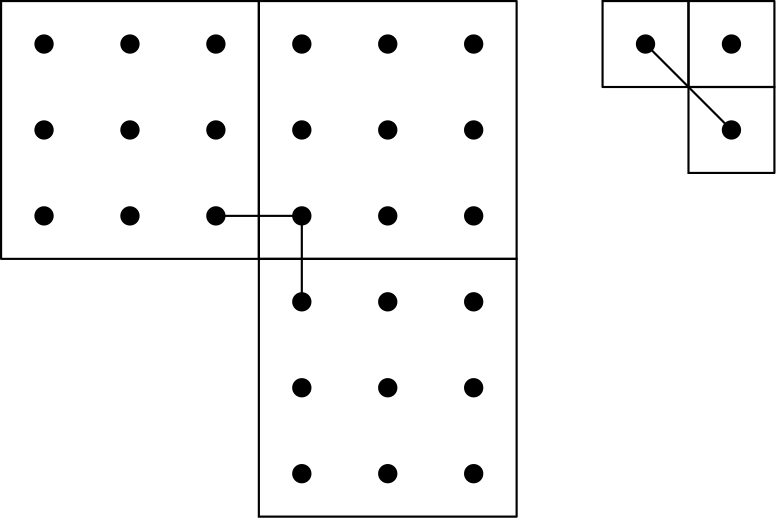
\includegraphics[width=0.5\textwidth]{figures/ising-2d-higher-order.png}
  \caption{In block RG, summing over corner spins induces next-nearest
    neighbors interactions. Subsequent iterations will introduce all
    possible couplings.\label{fig:ising-block-couplings} }
\end{figure}


This extends readily to any block size and number of dimensions, $d$:%
\begin{equation}%
  K'\approx b^{d-1} K;
\end{equation}%
for $b,d>1$, then, $K=\infty$ is locally stable. By differentiating
\fref{eq:ising-1d-recursion-relation-J}, around $K=0$, we see that
this point is also locally stable. Between these two stable fixed
points, then, we expect a critical point, evidence that our assumptions
were reasonable and that RG is an appropriate tool.


\subsubsection{Applying RG\@: Decimation}
In 1D, decimation is known to be the optimal procedure, that is, it
suppresses higher-order terms in subsequent hamiltonians. Although
decimation will not translate to higher dimensions, working through
the solution and comparing with our results by the transfer matrix
method will prove a worthwhile exercise. We will simplify by assuming
$0$-external field. In decimation, we perform a partial sum to
eliminate some fraction of the spins, chosen so as to render the
resulting lattice structure identical to the starting lattice
structure
\sref{fig:decimation}. % DON't KNOW if 'structure' is the right word but 'lattice' alone is misleading

\begin{figure}[ht]
  \centering
  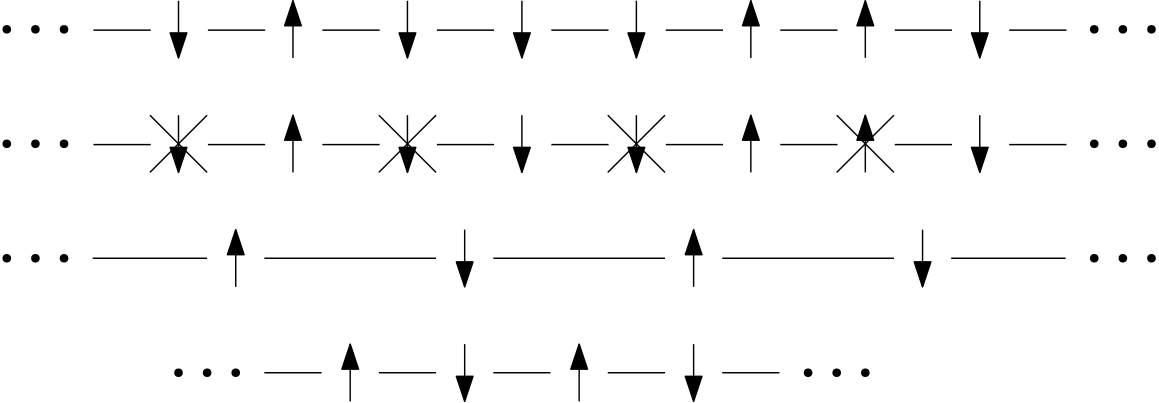
\includegraphics[width=0.5\textwidth]{figures/decimation.png}
  \caption{Decimation as applied to the Ising model in
    1D.\label{fig:decimation} }
\end{figure}

For computational ease, we take the number of spins to be
$2N$\footnote{We ultimately care about the limiting case that
  $N\rightarrow\infty$, so this is perfectly valid}:%
\begin{equation}%
  H(\bs)=-J\sum_{i=1}^{2N} s_i s_{i+1},
  \label{eq:ising-energy-fn-0-field}
\end{equation}%
again with periodic boundary conditions, where now $s_{2N+1}=s_1$. Our
transformation reads as:
\begin{equation}%
  e^{-H'(\bs')}=\sum_{s_2,s_4,\dots,s_{2N}} e^{-H(\bs')},
  \label{eq:decimation-transformation}
\end{equation}%
where $\bs'$ ranges over the odd coordinates. All odd spins are
allowed to vary independently so we can factor the above into
expressions relating adjacent spins in $J'$, for example, for the
first two spins:
\begin{equation}%
  g(J')e^{-J's_1 s3}=\sum_{s_2} e^{-J (s_1s_2+s_2s_3)}.
\end{equation}% MAYBE I SHOULD USE K = J/BETA??
From this equation, we can determine $J'$ and $g(J')$ in terms $J$. We
could, then, express the new Hamiltonian in a form almost identical
to~\pref{eq:ising-energy-fn-0-field}.

Solving the left-hand side~\cite{domb}: %
\begin{align}%
  \sum_{s_2} e^{-J (s_1s_2+s_2s_3)}&=2 \cosh {J (s_1+s_3)}\\
                                   &=e^{Js_1}e^{Js_3}+e^{-Js_1}e^{-Js_3}\\
                                   &=(\cosh J+s_1\sinh J)(\cosh J+s_3\sinh J)\\
                                   &\ +(\cosh J-s_1\sinh J)(\cosh J-s_3\sinh J)\\
                                   &=2\cosh^2 J(1+s_1s_2 \tanh^2 J).
\end{align}%
If we now input two different choices for $s_1$ and $s_3$, we can
determine $J'$: from %
\begin{align}%
  s_1=s_3=1:&\tab g(J')e^{-J'}=2\cosh 2J\\
  -s_1=s_3=1:&\tab g(J')e^{J}=2,
\end{align}%
it follows that %
\begin{align}%
  J'&= \frac{1}{2}\ln \cosh 2J \label{eq:ising-1d-recursion-relation-J}\\
  g(J')&=2\cosh^{1/2} 2J. \label{eq:ising-1d-recursion-relation-f}
\end{align}%
These are our transformation rules or recursion relations.

\paragraph{Free Energy.}
We still have to show that these transformations extract the
macroscopic information in the vicinity of the fixed points. By
invariance under choice of index, we can extend
\fref{eq:ising-1d-recursion-relation-J} to all spins
in~\fref{eq:decimation-transformation}:
\begin{equation}%
  2^N \cosh^{N/2}(2J) Z'(J')=Z(J).
\end{equation}%
In terms of the reduced free energy $f = F/N= (\ln Z)/N$, we can
reexpress the above as:%
\begin{equation}%
  \ln \left( 2 \cosh^{1/2}(2J)\right) + f(J')=2 f(J),\label{eq:decimation-f-transformation-0}
\end{equation}%
recalling that our original lattice had $2N$ sites and our
renormalized lattice has $N$ sites.

\paragraph{Fixed Points.}
If we look for fixed points,%
\begin{equation}%
  J=J^*=\frac{1}{2} \ln \cosh 2J^*,
\end{equation}%
we find only $J^*=0, \infty$. Indeed, we have confirmed that there is
No non-trivial critical pointfor the Ising model in 1D
\sref{fig:ising-1d-fixed-points}

\begin{figure}[ht]
  \centering
  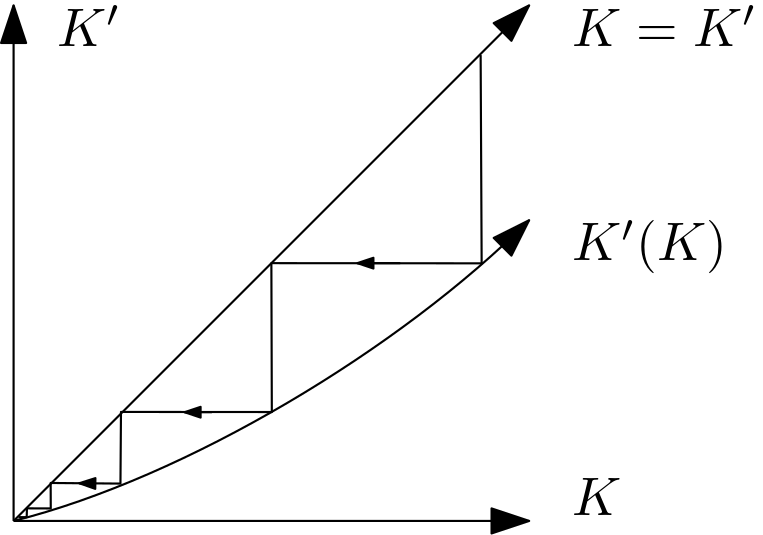
\includegraphics[width=0.5\textwidth]{figures/ising-1d-stability.png}
  \caption{Stability diagram for the Ising model in 1D. There are two
    fixed points, $J=0$ and $J=\infty$, the second of which is
    unstable. There is no intermediate critical point and no
    spontaneous temperature for any
    $J\neq 0$.\label{fig:ising-1d-fixed-points}}
\end{figure}

Let us now confirm that our predictions from RG line up with exact
results from \fref{sec:ising-1d-exact}. We will do this by looking at
the behavior of the free energy near the fixed points. Near these
points, the free energy is invariant under RG transformations:%
\begin{equation}%
  f(J)\approx f(J') \approx f(J^*)
\end{equation}% FIGURE OUT f' vs f, just be consistent

Plugging this in, we get:
\begin{equation}%
  f(J)\approx \ln \left( 2 \cosh^{1/2}(2J)\right)
\end{equation}%

At our critical points then:
\begin{align}%
  f(0)&\approx \ln 2\\
  f(\infty)&\approx J=\infty\\
  \label{eq:ising-1d-rg-free-energy}
\end{align}%

Comparing with \fref{eq:ising-1d-free-energy-at-fixed-pts}, we see
this lines up with the exact results. From this expression for the
free energy, we can extract the critical
exponents\label{sec:decimation-free-energy}. We will do for the case
of the 2d Ising model.
%
\subsection{Block RG Generalization}\label{sec:block-rg-generalization}




How might we use RG to derive predictions for critical exponents?
Consider the 1-dimensional Ising model. We can apply RG to this exactly, using
\textit{decimation}. Instead of performing a kind of average over blocks,
we simply take the value at the center of each block, and marginalize over the rest.
If we start with a Hamiltonian $H(\bs)=-K\sum_{ij}s_is_j$, then all subsequent
Hamiltonian's will be of a similar form: $H'(\bs')=-K'\sum_{ij}s_i' s_j'$.

Consider the example of correlation length, $\xi$, which we will
measure in terms of the lattice spacing, $a$, so it is
dimensionless. Then, it can depend only the couplings $\{K\}$: $\xi=xi\{K\}$.
After renormalization, the macroscopic properties of our system are same. The
dimensionful, $\xi$, should also be preserved. However, in our example, the coarse-graining
procedure increases the lattice spacing by a factor of $b=3$. We have to rescale,
and the dimensionless correlation length transforms as:
\begin{equation}%
\xi(\{K'\})=b^{-1}\xi(\{K\}).
\end{equation}%
We can solve this to get:
\begin{equation}%
\xi(\{K\})=\frac{\text{const.}}{\ln }
\end{equation}%






The coupling constants will depend on physical parameters like
temperature, pressure, external magnetic field in some, possible
complicated, way. In order for the experimentalist to bring a system
to the critical surface, they will have to adjust $n$ such
parameters. In the case of the Ising model, we require two such
parameters, temperature and external magnetic field. Indeed, its fixed
point has two relevant scaling variables. By symmetry arguments, we
see that one of these relevant temperature must be temperature-like,
\textit{thermal}, and the other \textit{magnetic}. The thermal scaling
variable, $u_t$, lies in the even subspace of couplings, and the
magnetic scaling variable, $u_b$, in the odd subspace. That the Ising
fixed point occurs at zero-field implies that the fixed point occurs
in the subspace that all odd-couplings vanish. Then, $\bolds{\mc{J}}$
contains no elements connecting either subspaces and its eigenvectors
are either odd or even according to the symmetry $s \rightarrow -s$.
\subsubsection{Correlation Length Critical Exponent}


Another example is the nearest neighbor correlation function, $C$,
which measures the tendency of neighboring spins to align with one
another, is expressed as a second derivative of the free energy with
respect to $J$:
\begin{equation}%
  C(s_i,s_j)=\expect{s_is_j}-\expect{s_i}\expect{s_j}=\partial_J^2 F.
\end{equation}%
With derivation:
\begin{align}
  \partial_J \left(-\log Z\right) &=-\partial_J\left(\frac{1}{Z}\sum_{\bs}\partial_J e^{-B \sum_i s_i - J \sum_{\expect{i,j}} s_i s_j} \right)\\
                                  &=-\partial_J\left(\sum_{\bs} \frac{e^{-E(\bs)}}{Z} \left(-\sum_{\expect{i,j}} s_i s_j\right)\right)\\
                                  &=\sum_{\bs}\left(\sum_{\expect{i,j}} s_i s_j\right)
                                    \left[\left(\partial_J e^{-E(\bs)}\right)\left(\frac{1}{Z} \right)-\left(e^{-E(\bs)}\right)\left(\partial_J \frac{1}{Z}\right)\right]\\
                                  &=\frac{1}{Z^2}\sum_{\bs}\left(\sum_{\expect{i,j}} s_i s_j\right)\left(\sum_{\bs} \sum_{\expect{i,j}} s_i s_j-\sum_{\bs'} \sum_{\expect{i,j}'} s_i' s_j'\right)\\
                                  &= \expect{s_i s_j}-\expect{s_i} \expect{s_j}.
\end{align}%

\

\section{RBM}
Let us begin by considering what, at first, seems like an unrelated
question. Consider a Markov random field, an undirected graphical
model of the kind depicted in \fref{fig:markov-random-field}. Nodes,
$v_i$, represent the variables, and connections between nodes denote a
conditional dependence between the corresponding two variables. We
will consider the case of binary-valued random variables:
$v_i \in \{0,1\}$\footnote{The ``Markov property'' means that a given
  variable's probability measure is entirely specified by its
  neighbors. Two variables that do not share a connection are independent.}.

\begin{figure}[ht]
  \centering
  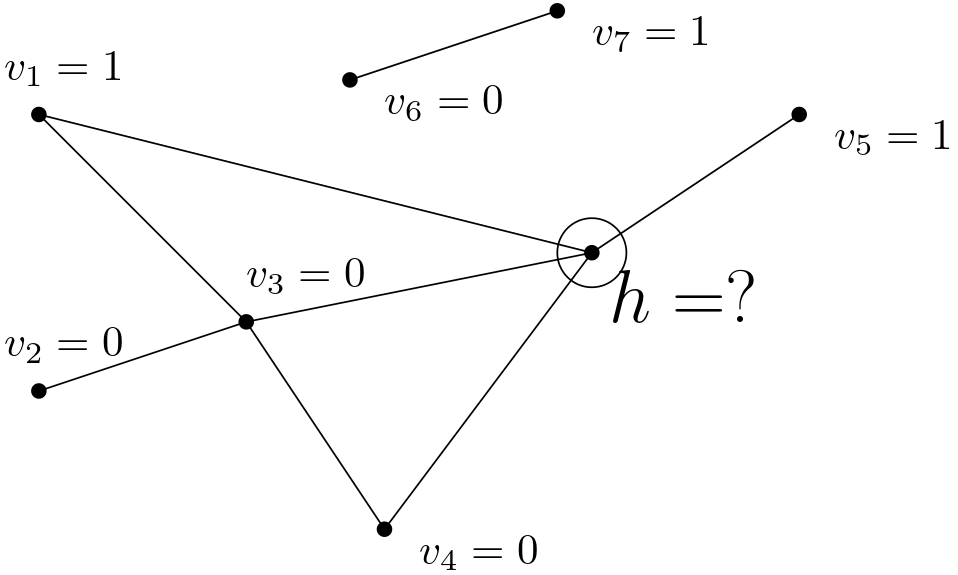
\includegraphics[width=0.5\textwidth]{figures/markov-random-field.png}
  \caption{An undirected Markov random field: nodes are random
    variables, and connections model conditional
    dependence.\label{fig:markov-random-field} }
\end{figure}

Our first question is: if we specify the state of all but one
variable, $v_i$, can we calculate the most likely value, the
expectation, of a remaining variables, $h$ (this is the conditional
probability $P(h|\bv)$? Here, we call the inputted variables
\textit{visible} and the unknown variables
\textit{hidden}\footnote{This should remind you of the terminology we
  used with renormalization.}. Let us first consider the case of
learning a single hidden variable, having specified all others.

The simplest case is that of a linear interdependence; the value of
node $h$ depends on $v_i$ according to some weighting $w_{ij}$ plus a
bias $b$ that acts as a threshold for activation
\fref{fig:perceptron}. To ensure that the result of this linear
transformation is in $[0,1]$ (as is required for probabilities), we
run it through a sigmoid function \pref{fig:sigmoid}:

\begin{equation}%
  \sigma(x)=\frac{e^x}{1+e^x}=\frac{1}{1+e^{-x}}
\end{equation}%

Our probability for $h$ given a configuration of visibles, $\bv$ is:
\begin{equation}%
  P(h|\bv)=\sigma(h)=\frac{1}{1+e^{-h(\sum_i w_{ij} v_i - b )}}
\end{equation}%

\begin{figure}[ht]
  \centering
  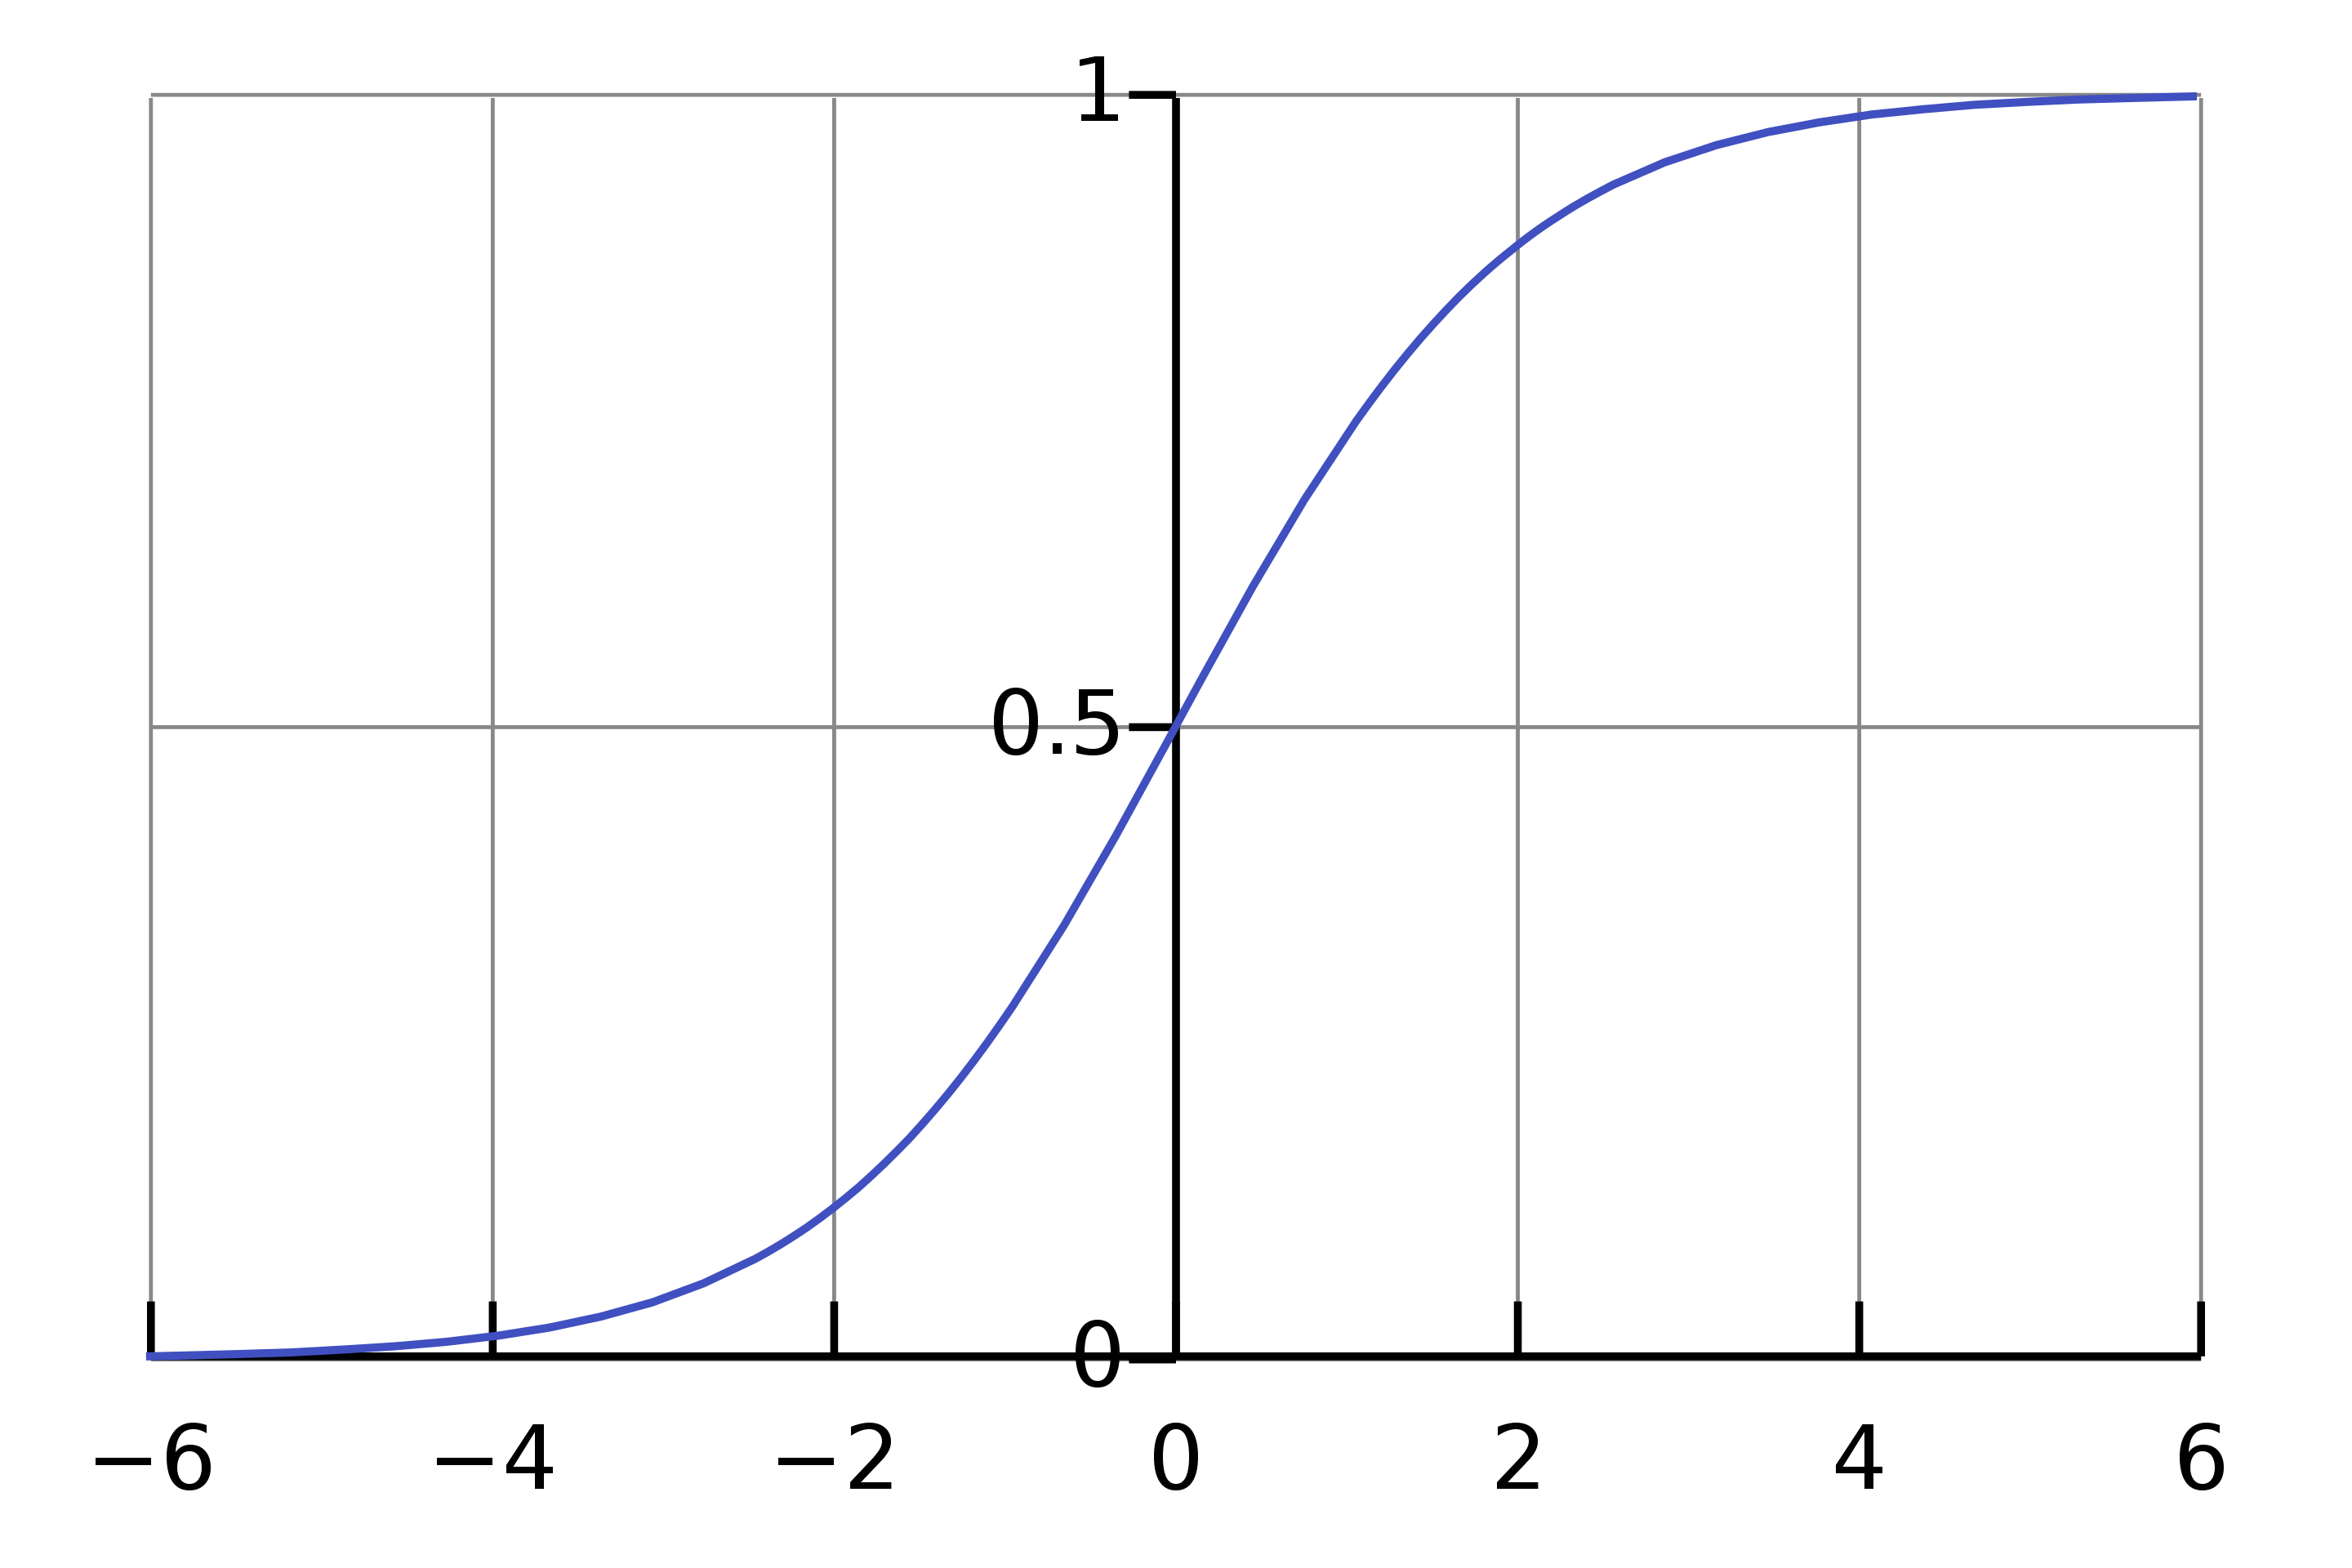
\includegraphics[width=0.5\textwidth]{figures/sigmoid.png}
  \caption{The sigmoid function, $\sigma(x)$ (Image: Qef via Wikimedia Commons~\cite{sigmoid}).\label{fig:sigmoid.png} }
\end{figure}

\begin{figure}[ht]
  \centering
  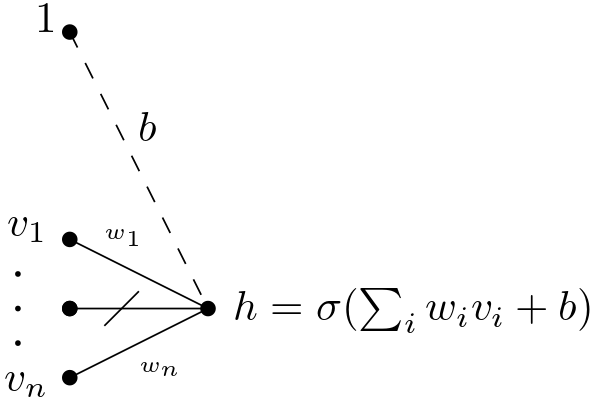
\includegraphics[width=0.5\textwidth]{figures/perceptron.png}
  \caption{A hidden unit taking input from one and multiple visible
    units.\label{fig:perceptron} }
\end{figure}

We can naturally extend this to the task of inferring the states of
multiple hidden units $\bh=\seth_{j=1}^M$, simply repeating the above
procedure for every hidden node in turn. Complications arise when we
consider hidden nodes that depend on other hidden units. To avoid this
scenario, we consider a restricted set of graphs, those without
connections between hidden nodes. We get that the conditional
probability for an entire layer of hiddens is:%
\begin{equation}%
  P(\bh|\bv)=\prod_{j=1}^M \sigma(h_j)=\prod_{j=1}^M \frac{1}{1+e^{-h_j(\sum_i w_{ij} v_i - b_j )}}
\end{equation}%

If we restrict ourselves further, to graphs without connections
between visible units, we can conduct statistical inference in both
directions: given a sample of visible units we can measure
expectations or sample possible hidden states, and
vice-versa\footnote{The distinction between ``visible'' and ``hidden''
  no longer refer to the direction of inference (inference can go both
  ways).  Instead, we often use ``visible'' to refer to raw data, and
  ``hidden'' to higher-level, coarse-grained information.  We will
  make this more precise in the next subsections. Typically, at least
  in the examples we consider, the hidden layer will consist of less
  units than the visible layer.} \sref{fig:rbm}. This constitutes a
``restricted'' Boltzmann machine (RBM). If we denote the biases of the
visible units as $\{a_i\}$, we get that the conditional probability of
a layer of visibles given a layer of hiddens is:%

\begin{equation}%
  P(\bh|\bv)=\prod_{j=1}^M \sigma(h_j)=\prod_{j=1}^M \frac{1}{1+e^{-h_j(\sum_i w_{ij} v_i - b_j )}}
\end{equation}%

\begin{equation}%
  P(\bv|\bh)=\prod_{i=1}^N \sigma(v_j)=\prod_{i=1}^N \frac{1}{1+e^{-v_i(\sum_j w_{ij} h_j - a_i )}}
\end{equation}%

\begin{figure}[ht]
  \centering
  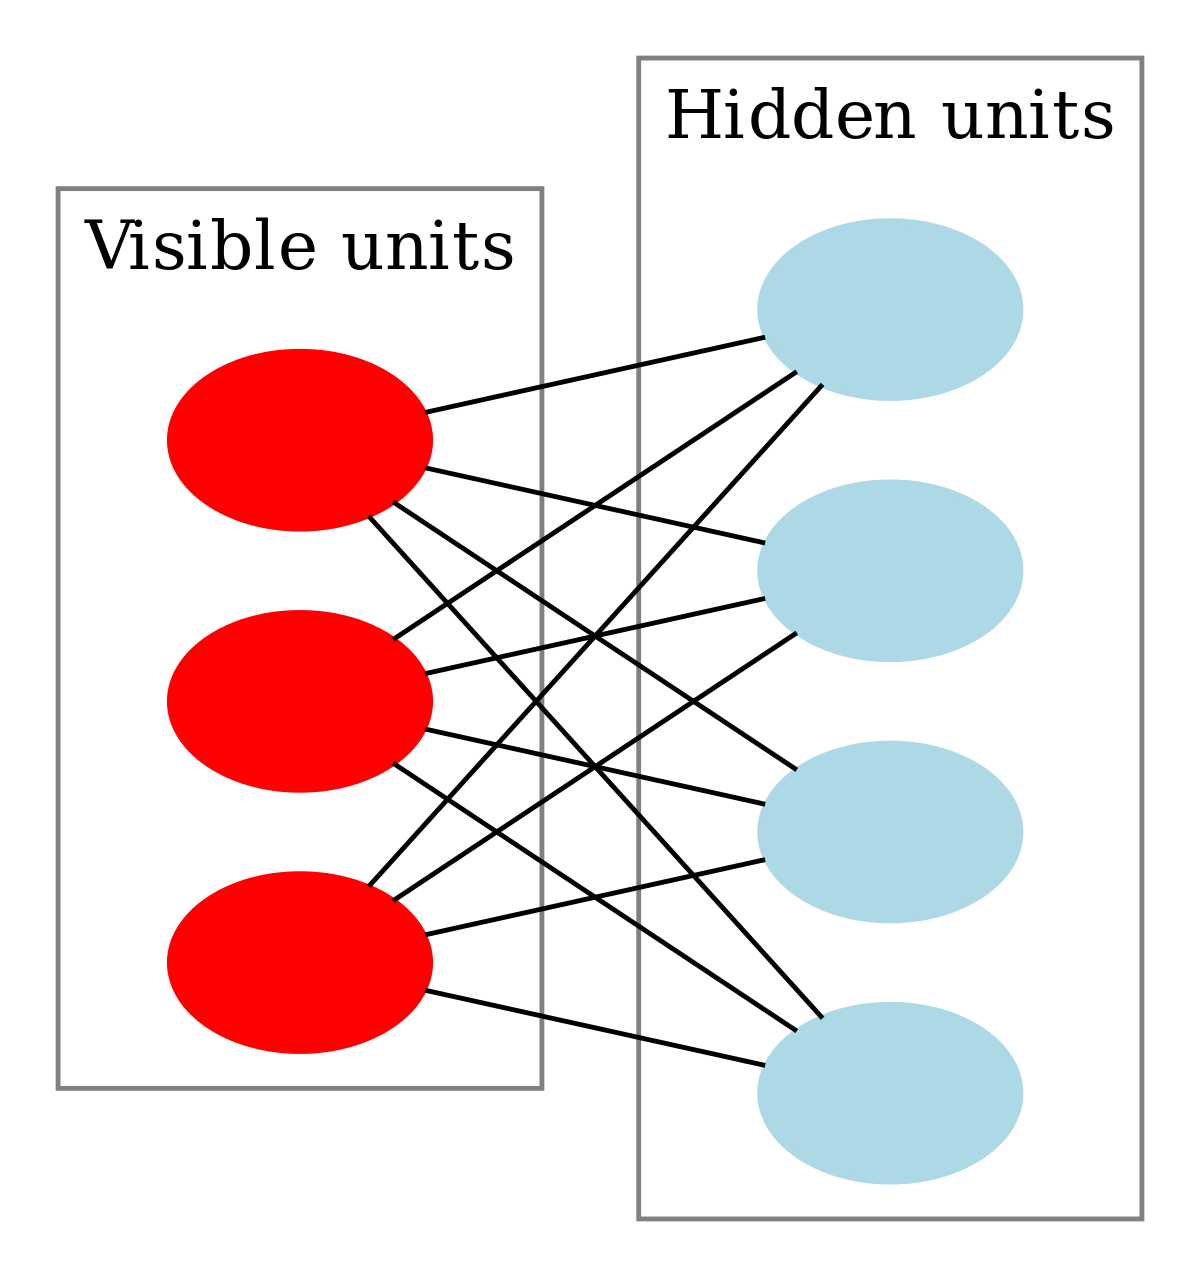
\includegraphics[draft, width=0.5\textwidth]{figures/rbm.png}
  \caption{A restricted Boltzmann machine: an undirected Markov random
    field with a bipartite structure. This has an alternate
    interpretation as an artificial neural network.\label{fig:rbm} }
\end{figure}

This Markov random field has an alternate interpretation as an
artificial neural network. We approximate biological neurons as
binary-valued values: on and firing, or off and waiting. In a given
time step, a neuron will probabilistically fire, depending on the
behavior of its neighbors. Again, we approximate their connections as
linear (\sref{fig:rbm}).


\subsection{Conditional Probabilities}\label{sec:rbm-conditional-dist}

Conditional probs



\subsubsection{Derivatives of Kullback-Leibler
  Divergence}\label{sec:kld-differentiation}

\begin{align}
  \partial_\l H(P_{true}(\bx),P_\l(\bx))
  &= \partial_\l\left(\sum_{\bx}P_{true}(\bx)\ln(P_\l(\bx))\right) \\
  &=\sum_{X}\left((\partial_\l P_{true}(\bx))\ln(P_\l(\bx)) + \frac{P_{true}(\bx)}{P_\l(\bx)} \partial_\l P_\l(\bx)\right)\\
  &=\sum_{X}\frac{P_{true}(\bx)}{P_\l(\bx)} \partial_\l P_\l(\bx)
\end{align}

This is equivalent to minimizing the negative log-likelihood of

\subsection{Regularization}\label{sec:regularization}


\section{RSMI}
\subsection{Approximating Mutual Information}
\subsection{Derivative of Mutual Information Proxy}\label{sec:rsmi-derivation}


\subsection{Exact: Decimation for the 1D Ising Chain}
Consider the geometry depicted in \fref{fig:rsmi-decimation}. A block
region $\bv=\{v_1\dots,v_{L_\bv}$ of size $L_\bv$ surrounded by a
buffer region, $\bb=\{b_{-L_\bb}\dots,b_{-1},b_1\dots,b_{L_\bb}$, of
size $2L_\bb$, an environment,
$\be=\{e_{-L_\be}\dots,e_{-1},e_1\dots,e_{L_\be}$ of size $2L_\be$,
and the rest of the system, $\bo$. We assume that $L_\bb+L_\be$ is
much larger than the correlation length, so we can discard the rest of
the system in subsequent calculations. Here we can exactly calculate
the probability distributions $P(\bv)$ and $P(\bv,\be)$ that show up
in our expression for the mutual information. We again use the
transfer matrix formalism, where now we assume $0$-magnetic field:
\begin{equation}%
  Z=\Tr \bT^N={(2\cosh(K))}^N\rvert_{B=0},\tab
  \bT=
  \begin{array}
    e^K & e^{-K} \\
    e^{-K} & e^{K} \\
  \end{array}.
\end{equation}%
For $P(\bv)$, we get:
\begin{align}%
  P(\bv)=\sum_{\bb,\be,\bo}P(\bx)&=\sum_{\bb,\be,\bo}\frac{\prod_i^N T_{x_i,x_{i+1}}}{Z}\\
                                 &=\frac{1}{{(2\cosh(K))}^{L_\bv+1}}\sum_{b_{-1},b_{1}}T_{b_{-1},v_1}T_{v_1,v_2}\dots T_{v_{L_{\bv}-1},v_{L_{\bv}}}T_{v_{L_{\bv}}, b_{1}}.
\end{align}%

With similar calculations, we get:%
% \begin{equation}%
%   P(\bv,\be)=\frac{1}{{(2\cosh(K))}^{L_\bv+2L_\bb+2L_\be+1}}\sum_{o_{-1},o_{1}}T_{o_{-1},e_{-L_{\be}}}T_{e_{-L{\be}},e_{-L{\be}+1}}\dots T_{e_{-1},v_1}^{L_\bb+1}T_{v_1,v_2}\dots T_{v_{L_{\bv}},e_1}^{L_\bb+1}T_{e_1,e_2}\dots{e_{L_{\be}}}, o_{1}}.
% \end{equation}

If we try to write these equations in terms of a Boltzmann
distribution, we'd get the energy functions:%
\begin{align}%
  E(\bv)&=-\sum_{i=1}^{L_\bv}Kv_i v_{i+1} + const.\\
  E(\bv,\be)&=-\sum_{i=1}^{L_\be}Ke_i e_i+1 - K_{L_\bb}(e_{-1}v_1+v_{L_\bv}e_1)+E(\bv)+ const'.\\
  \Delta E(\bv,\be)= E(\bv,\be)-E(\bv)=-\sum_{i=1}^{L_\be}Ke_i e_i+1 - K_{L_\bb}(e_{-1}v_1+v_{L_\bv}e_1)+ const''.
\end{align}%

The constant terms arise from the boundary interactions, and
$K_{L_\bb}$ is the effective interaction through $\bb$ between the
visible and environmental boundary spins (from
$T_{e_{-1},v_1}^{L_\bb+1}$ and $T_{v_{L_\bv},e_1}^{L_\bb+1}$).

We can, now, solve for the mutual information proxy:
\begin{equation}%
  A_{\L}(\bh,\be)\approx \sum_{\bh,\bv,\be}P(\bv,\be)P_\L(\bh\rvert\bv)\expect{-\delta E(\bv,\be)}[\be, \bh].
\end{equation}%

Remember that the expectation value of $\Delta E(\bv,\be)$ is
evaluated over $\bv'$. Then, we can remove any terms which do not
involve $\bv$ from inside the expectation value (for example,
$\expect{Ke_1e_2}=Ke_1e_2$). We can also remove any constant terms, as
these have zero-derivative.  The mutual information reduces to:%
\begin{equation}%
  A_{\L}(\bh,\be)\approx \sum_{\bh,\bv,\be}P(\bv,\be)P_\L(\bh\rvert\bv)\expect{K_{L_\bb}(e_{-1}v_1+v_{L_\bv}e_1)}[\be, \bh].
\end{equation}%
p
MORE DETAILS
One idea would be to keep our linear transformations (leave the RBM's
energy function unchanged), but change the non-linearity function. For
example, if $n=3$ (so spins can take values in $\{-1,0,1\}$), then,
instead of running the result through a sigmoid, we might run it the
following:%
\begin{equation}%
  \sigma_{(3)}(x)=-1+ \sigma(x+a)+\sigma(x-a),
\end{equation}%
which is plotted in \fref{fig:ternary-sigmoid} along with its
derivative.

\begin{figure}[ht]
  \centering \includegraphics[]{figures/ternary-sigmoid.png}
  \caption{The ternary sigmoid for $a=5$ and its
    derivative\label{fig:ternary-sigmoid.png}.}
\end{figure}

From the derivative, we see that the stable values of our neurons
under gradient descent are $-1$,$0$, and $-1$, exactly as we
wanted. If we want to regain stochasticity, we can use a rule like%
% \begin{align}%
%   P(h_j=1|\bv)=\begin{array}
%                  \sigma_{(3)}(a_j)} \text{ if } a_j> 0 \\
%                  0 & \text{otherwise.}
%                \end{array}\\
%                %   P(h_j=-1|\bv)=\begin{array}
%                   -\sigma_{(3)}(a_j)} \text{ if } a_j< 0 \\
%                   0 & \text{otherwise.}
%                 \end{array} \\
%                 %   P(h_j=0|\bv)=1-P(h_j=1|\bv)-P(h_j=-1|\bv),
% \end{align}%
where $a_j=\sum_i w_{ij} v_i+b_j$ (the activation of h).

The above fails, however, when the values neurons can take (the spins)
are not linearly ordered. According to the above, a spin of $-1$ would
be more similar to $0$ than to $1$. Of course, we can easily conceive
of Hamiltonian's where this is not the case. For example, consider
\begin{equation}%
  H(\bx)=\sum_{\expect{ij}} K^{(0)} x_i^2 x_j^2+\sum_{i} K^{(1)}x_i^2
\end{equation}, a Hamiltonian which is perfectly symmetrical under $-1\arrow 1$. This might represent an alloy of two compounds with vacancies. The two compounds do not experience an interaction energy but there is an interaction between vacancies and neighboring particles. In fact, this Hamiltonian is exactly equivalent to the Ising model
under $-1\rightarrow 1, 0\rightarrow -1$. Evidently, $n$-ary neurons of the above type are inappropriate for the task at hand.


\section{Information theory}\label{sec:information-theory}





Koch-Janusz and Ringel claim that the RSMI algorithm learns
``optimal'' RG transformations. ``Optimal'' would mean that successive
Hamiltonians are as compact as possible.


Their formal requirement is that the Taylor-expansion of the effective
Hamiltonian, $\bH'$, at successive steps is as compact as possible:%
\begin{equation}%
  \bH'=\sum_i K^{(0)}h_i+\sum_{\expect{i,j}} K^{(1)}h_i h_j +\sum_{\expect{\expect{i,j}}}K^{(2)}h_i h_j + \sum_{\expect{i,j,k}}K^{(3)} h_i h_j h_k + \dots
\end{equation}%
In other words, this expansion should contain only short-ranged and
few-body terms; the coefficients $K^{(n)}$, should decay exponentially
with distance. Having satisfied these requirements, we can discard
terms past some distance without majorly affecting the state of the
system $\bh$. As Koch-Janusz and Ringel go on to say, the above
formulation makes it intuitively clear what constitutes a suitable RG
scheme but is typically hard to formalize. The RSMI algorithm, on the
other hand, is precise and computationally implementable. In fact,
they claim, the two formulations are equivalent. Maximizing the mutual
information encourages the hidden variables to couple to the
combinations of $\bv$ most strongly correlated with the environment.
These are simply the most relevant operators in the theory at a given
level and are the basic fields that manifest in the low-energy (i.e.\
macroscopic) theories\marginpar{Simplify the above and make it more
  fitting, clearer pivot to the following.}.



\subsection{Measuring ``Temperature'' Evolution}




    To use this technique for estimating macroparameters, we
will need to train different RBMs for each temperature. Otherwise, we
would have no way of knowing the samples it generates are related in
any way. So we still need labels.  This seems to contradict our claim
that this example is unsupervised.  Indeed, the distinctions are, at
times, less clear. We will get back to this point as it has led to
some confusion in the literature. Suffice to say that the models
themselves do not encounter any labels during
training.\footnote{Interestingly, Iso et al.\ showed that Gibbs
  sampling performed by RBMs trained on a range of temperatures
  produced samples \textit{at} the critical temperature. Temperatures
  seem to flow towards the critical point rather than away, as in
  RG\@. The authors misleadingly conclude that RG is the opposite of
  RBMs. In fact, this comparison is inappropriate. These RBMs perform
  nothing like RG, and the authors are comparing apples and
  oranges. For more see \fref{sec:relevant} on the role of relevant
  information.}


Let us consider only the argument of the exponential in the
denominator, choosing $b_j=0$:
\begin{equation}%
  -h_j\sum_i w_{ij} v_i.
\end{equation}%
Let us split the components of $v_i$ into two separate groups, indexed
by $i'$ and $i''$. Where $i \in \{1\ldots N\}$, now
$i'\in\{1\ldotsN/2\}$ and $i''\in\{1\ldotsN/2\}$. How we make this
split is not important, it could be purely random.\footnote{This
  correspondence only works for even-block renormalization} Then, the
term becomes:
\begin{equation}%
  -h_j(\sum_{i'} w_{i'j} v_{i'} +\sum_{i''} w_{i''j} v_{i''}).
\end{equation}%
The trick will be to let half of $w_{ij}$ components be negative and
the other half positive.  We introduce a simpler parameter $w$, so
that $w_{i'j}\eqcolon w$ and $w_{i'j}\eqcolon -w$.  Then, we get:
\begin{equation}%
  -h_j w(\sum_{i'}v_{i'} -\sum_{i''} v_{i''}).
\end{equation}%
Note that the term $\sum_{i'}v_{i'} -\sum_{i''} v_{i''}$ is positive
precisely when $\expect{v_i}>1/2$, and negative (or zero) otherwise.
If we fix the sign of $w$, then this
Let us summarize what we have accomplished.  We began overviewing the
basic elements of statistical physics, which has the goal of turning
microscopic theories into concrete macroscopic observables. To do
this, one requires a probability distribution over microstates, and
from a small set of assumptions, one can derive this
distribution. This, however, leads to a divergence, and we explored
the range of tools available.

We glimpsed at MCMC methods: instead of calculating full sums, one can
average over representative samples, replacing a calculation of
absolute probabilities with iterative rules of relative probabilities.

The limitations of MCMC methods brought us to mean-field theory. Here,
one replaces the absolute probability with a series of conditional
probabilities over individual spins. Imposing a restriction on these
conditional probabilities, one can calculate magnetization and
correlation lengths. This method failed below four dimensions though
it offers valuable insights: the existence of a critical point, a
divergence of the correlation length, and a preview of critical
exponents.

We sampled a set of more powerful techniques: the renormalization
group.  Instead of solving the partition function outright, one can
iteratively simplify it, transforming a system's information to a
manageable form. Working out the consequences, one encounters
universality: how many seemingly different systems are macroscopically
indistinguishable. From, the RG eigenvalues one determines critical
exponents and relations between exponents. To compute these eigenvalues,
we explained several approximations: the~$4-\epsilon$, borrowing perturbative
techniques from QFT\@; MCMC techniques, now embracing their
finite-size limits; finally, Kadanoff's technique, controlling the
evolution of parameters with variational bounds on the free
energy. However, we saw that devising suitable transformations was
challenging, lacking rigor and generality.

In \fref{sec:ml}, we turned to ML\@. Whereas statistical physics is
concerned with estimates over populations of samples, ML prefers
working with individual samples. This manifested in our first
demonstration where we used an RBM to classify phases.  Then, we
considered training RBMs to generate new samples of Ising
models. These examples presented several qualitative similarities
between ML and RG\@.

on the architecture of the models (as convolutional neural networks).

In \fref{sec:rsmi}, we adapted our new notion of ``relevance'' to the
physical setting where relevant is long-distance information. This
brought us to a general criterion for appropriate RG procedures on
lattices. With Koch-Janusz and Ringel's variational proxy, we were
able to train an ML algorithm to learns such transformations without
supervision.

In \fref{sec:validation}, we used this algorithm to calculate the
correlation length critical exponent. Reviewing the RSMI algorithm, we
elaborated on a number of possibilities for the future: a
generalization to other systems and the introduction of more powerful
models of the probabilities. We reflected on the possibility of using
other calculations of mutual information and identified interesting
contemporary research within ML\@.
